\documentclass{beamer}
\title{Team W - Algorithms for Sports Eliminations}
\author{
    Gordon Reid: 1002536R\\
    Ryan Wells: 1002253W\\
    Kris Stewart: 1007175S\\
    David Selkirk: 1003646S\\
    James Gallagher: 0800899G\\
    Dr David Manlove: Project Supervisor
}
\date{March 19, 2013}
\begin{document}
\frame{\titlepage}
\frame{\tableofcontents}
\section{Project outline}
\section{Progress so far}
\subsection{Algorithm - Gordon Reid and Ryan Wells}
\subsection{Parser - Kris Stewart and James Gallagher}
\subsection{User Interface - David Selkirk}
\frame{
  \frametitle{Project outline}
  \begin{itemize}
  \item<2-> Aim of the project is to implement an algorithm that
  will be able to say if a team X cannot win the Baseball league.
  \item<3-> Ford-Fulkerson algorithm used.
  \item<4-> A team X is only eliminated if there is no mathematically possible
  way for X to finish top of the league.
  \item<5-> Builds on na\"{\i}ve calculations made by sports pundits.
  \item<6-> Real world application of Graph Theory.
  \end{itemize}
}
\frame{
  \frametitle{Example}
  \begin{center}
  \begin{figure}
  %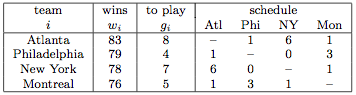
\includegraphics[width=\textwidth]{Example.png}
  \end{figure}
  \tiny{Image courtesy of Kevin D. Wayne, Princeton University}
  \end{center}
}
\frame{
  \frametitle{Algorithm}
  \pause
  \begin{center}
  \begin{figure}
  %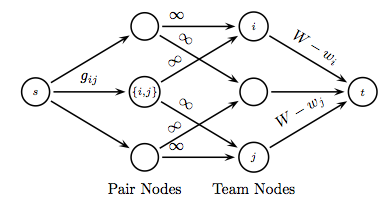
\includegraphics[width=0.4\textwidth]{graph.png}
  \end{figure}
  \tiny{Image courtesy of Kevin D. Wayne, Princeton University}
  \end{center}
  \begin{itemize}
  \item<2-> Revolves around creation of graphs and the flow along them.
  \item<3-> Pushing flow through the graph will allow us to determine if the
  given team X is eliminated from the league.
  \item<4-> A team X can win the league if it is possible for there to be a
  saturating flow. A flow is saturated if the total flow from the source equals
  the total capacity from the source.
  \item<5-> All flow leaving the source has to arrive at the sink.
  \item<6-> Currently can create all graphs and pushes flow along a
  particular graph.
  \end{itemize}
}
\frame{
  \frametitle{Parser}
  \pause
  \begin{center}
  \begin{figure}
  %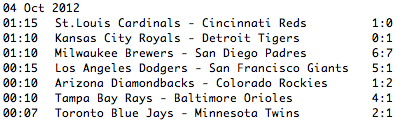
\includegraphics[width=\textwidth]{textfile.png}
  \end{figure}
  \end{center}
  \begin{itemize}
  \item<2-> Uses basic string comparison to put the relevant team in the
  correct League and Division.
  \item<3-> Have considered future plans to parse a web page.
  \item<4-> Our current source is not suitable for real-time updating.
  \item<5-> As a team we are unsure if we would like to implement this feature
  or concentrate our energies on other features for example, making a web-based
  UI.
  \end{itemize}
}
\frame{
  \frametitle{User Interface}
  \begin{itemize}
  \item<2-> Simple design based on presenting key information immediately.
  \item<3-> More detailed information available on user request.
  \item<4-> Challenge is to integrate the two tasks such that the UI is
  both functionally and aesthetically pleasing.
  \end{itemize}
}
\frame{
  \frametitle{User Interface - Key Tasks}
  \begin{itemize}
  \item<1-> Display all teams by division, league or elimination status.
  \item<2-> Update the elimination status on startup, as well as on week
  changes.
  \item<3-> Display certification of elimination for teams eliminated.
  \end{itemize}
}
\frame{
  \frametitle{User Interface - Prototype}
  \begin{figure}
  %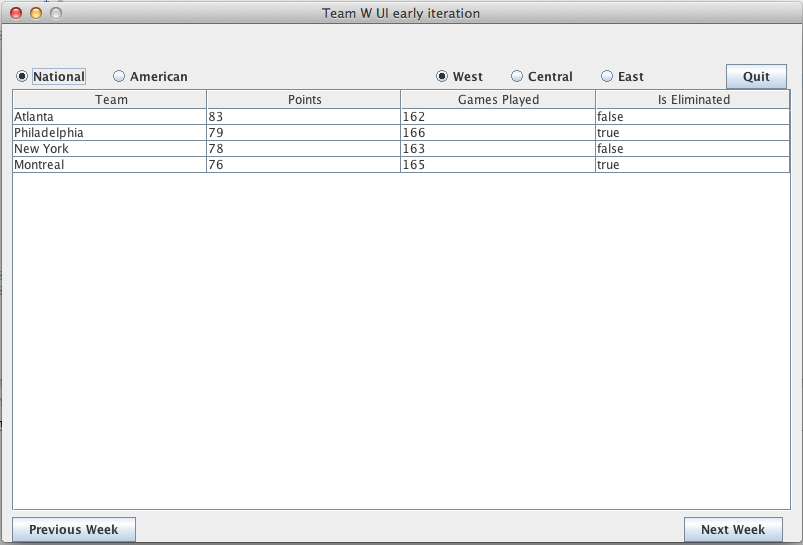
\includegraphics[width=\textwidth]{InitialUI.png}
  \end{figure}
}
\end{document}
